\documentclass[12pt, a4paper]{article}

\usepackage[T1]{fontenc}
\usepackage[utf8]{inputenc}
\usepackage[italian]{babel}
\usepackage{graphicx}
\usepackage{geometry}
\usepackage{xcolor}
\usepackage{setspace}
\usepackage{fancyhdr}
\usepackage{svg}
\usepackage{array}
\usepackage{lastpage}
\usepackage{caption}
\usepackage{xparse}
\usepackage[colorlinks=true, linkcolor=black, citecolor=blue, urlcolor=blue]{hyperref}

\renewcommand{\contentsname}{Indice}
\renewcommand{\sectionmark}[1]{\markboth{#1}{#1}}

\pagestyle{fancy}
\fancyhf{}
\fancyhead[L]{\nouppercase{\leftmark}}
\fancyhead[R]{pagina \thepage\ di \pageref*{LastPage}}

\geometry{
	top=2.5cm,
	bottom=2.5cm,
	left=3cm,
	right=3cm
}

% Spacing between figure and surrounding text
\setlength{\textfloatsep}{20pt}
\setlength{\intextsep}{20pt}

% Caption style (optional tweaks)
\captionsetup{
	font=small,
	labelfont=bf,
	skip=6pt
}

% Save originals before redefining
\let\origincludegraphics\includegraphics
\let\origincludesvg\includesvg

% Redefine \includegraphics[options]{file}{optional caption}
\RenewDocumentCommand{\includegraphics}{O{width=\linewidth} m g}{%
	\begin{figure}[htbp]
		\centering
		\origincludegraphics[#1]{#2}%
		\IfValueT{#3}{\caption{#3}}%
	\end{figure}%
}

\NewDocumentCommand{\insertsvg}{O{width=\linewidth} m g}{%
	\begin{figure}[htbp]
		\centering
		\let\includegraphics\origincludegraphics% prevent nested figure
		\includesvg[#1, inkscapelatex=false]{#2}%
		\IfValueT{#3}{\caption{#3}}%
	\end{figure}%
}

\renewcommand{\abstractname}{Sommario}

\begin{document}
	
	\begin{titlepage}
		\centering
		
		\origincludesvg[width=0.45\textwidth]{assets/logoUnisa.svg}
		
		\vspace{4cm}
		
		{\Huge\bfseries Metodologie Utilizzate PT}
		
		\vspace{0.6cm}
		
		{\LARGE\color{gray} Academy -- Cybersecurity}
		
		\vspace{2.5cm}
		
		{\large Kioptrix Level 1}
		
		\vspace{1.6cm}
		
		{\Large\bfseries Gruppo 15}
		
		\vspace{0.6cm}
		
		\begin{tabular}{>{\raggedleft\arraybackslash}p{6cm}@{\;--\;}p{6cm}}
			0612709539 & Francesco Cangianiello \\
			0612709671 & Andrea Ciliberti \\
			0612709638 & Serena Fierro \\
		\end{tabular}
		
		\vfill
		
		{\small A.A. 2025/2026}
		
	\end{titlepage}
	
	\newpage
	\thispagestyle{empty}
	\begin{abstract}
		Questo progetto mira a eseguire un'attività di Penetration Testing utilizzando la macchina virtuale "Kioptrix: Level 1". L'attività segue le fasi standard del framework FGPT, quali Target Scoping, Information Gathering, Target Discovery, Target Enumeration, Vulnerability Analysis, Target Exploitation, Privilege Escalation e Maintaining Access.
		Il progetto prevede l'emulazione di due macchine virtuali, poste nella medesima rete locale virtuale per permettere una connessione diretta, sfruttando i sistemi di virtualizzazione QEMU con tecnologia KVM. La macchina attaccante è una Kali Linux 2026.1, mentre la macchina attaccata si tratta della VM vulnerabile "Kioptrix: Level 1".
		
		Lo scopo del progetto è di verificare la sicurezza della macchina attaccata utilizzando tecniche e strumenti di Penetration Testing etico, individuando le vulnerabilità presenti sulla macchina target e proponendo soluzioni di rimediazione.
		
		Il presente documento mostra gli strumenti utilizzati e i passi seguiti per il completamento del progetto, proponendo una guida per la riproducibilità del processo di Penetration Testing e un'esposizione tecnica dettagliata del lavoro.
	\end{abstract}
	
	
	\newpage
	\thispagestyle{empty}
	\tableofcontents
	
	\newpage
	\section{Introduzione}
	\subsection{Fasi di lavoro}
	L'obiettivo finale del lavoro di Penetration Testing commissionato è di ottenere accesso remoto alla macchina target come amministratore (utente \texttt{root}).
	
	È stato seguito il framework FGPT per la scomposizione in passi del progetto, diviso nelle seguenti fasi:
	\begin{enumerate}
		\item \textbf{Target Scoping}: Definizione del perimetro di attività, studio
		delle regole di engagement e configurazione dell'ambiente di laboratorio.
		Include la pianificazione degli strumenti e delle metodologie da adottare
		nel corso delle fasi successive.
		
		\item \textbf{Information Gathering}: Raccolta di informazioni sulla macchina
		target da fonti pubblicamente disponibili, senza interagire direttamente con
		essa. L'obiettivo è costruire un profilo del sistema per pianificare una
		strategia di attacco più mirata.
		
		\item \textbf{Target Discovery}: Individuazione della macchina target
		all'interno della rete, senza conoscerne a priori le informazioni di rete.
		Si utilizzano tecniche di scansione ARP e di rete per identificare gli host
		attivi nella sottorete.
		
		\item \textbf{Target Enumeration}: Mappatura delle porte aperte, dei servizi
		esposti e del sistema operativo della macchina target. Fornisce le
		informazioni necessarie per delineare la superficie di attacco e orientare
		la ricerca delle vulnerabilità.
		
		\item \textbf{Vulnerability Analysis}: Identificazione delle vulnerabilità
		note sui servizi e sul sistema operativo rilevati, mediante strumenti
		automatici e ricerca manuale. L'obiettivo è individuare i vettori di attacco
		più critici da sfruttare nelle fasi successive.
		
		\item \textbf{Target Exploitation}: Sfruttamento delle vulnerabilità
		identificate per ottenere un accesso non autorizzato alla macchina target.
		Dimostra concretamente la presenza e l'impatto reale delle vulnerabilità
		sul sistema.
		
		\item \textbf{Privilege Escalation}: Elevazione dei privilegi da utente
		limitato ad amministratore di sistema (\texttt{root}), quando l'accesso
		iniziale ottenuto è insufficiente per raggiungere l'obiettivo. Completa
		il percorso di compromissione totale della macchina target.
		
		\item \textbf{Maintaining Access}: Installazione di meccanismi persistenti
		per garantire l'accesso remoto anche successivamente alla correzione delle
		vulnerabilità sfruttate. Simula le tecniche adottate da attaccanti reali
		per mantenere il controllo del sistema compromesso.
	\end{enumerate}
	
	Il setup del lavoro progettuale si è basato sullo studio delle regole di engagement del progetto, che includevano le informazioni di installazione della macchina su VulnHub e la necessità di dover strutturare una rete di test virtuale con collegamento diretto tra la macchina di attacco e macchina attaccata.
	
	\subsection{Architettura del laboratorio di test}
	Per configurare l'ambiente di laboratorio con le due macchine virtuali, si è fatto uso di QEMU/KVM su ambiente Linux. È stata configurata una rete LAN virtuale, connessa alla rete esterna tramite bridge NAT, all'intervallo di indirizzi 192.168.122.0/24.
	
	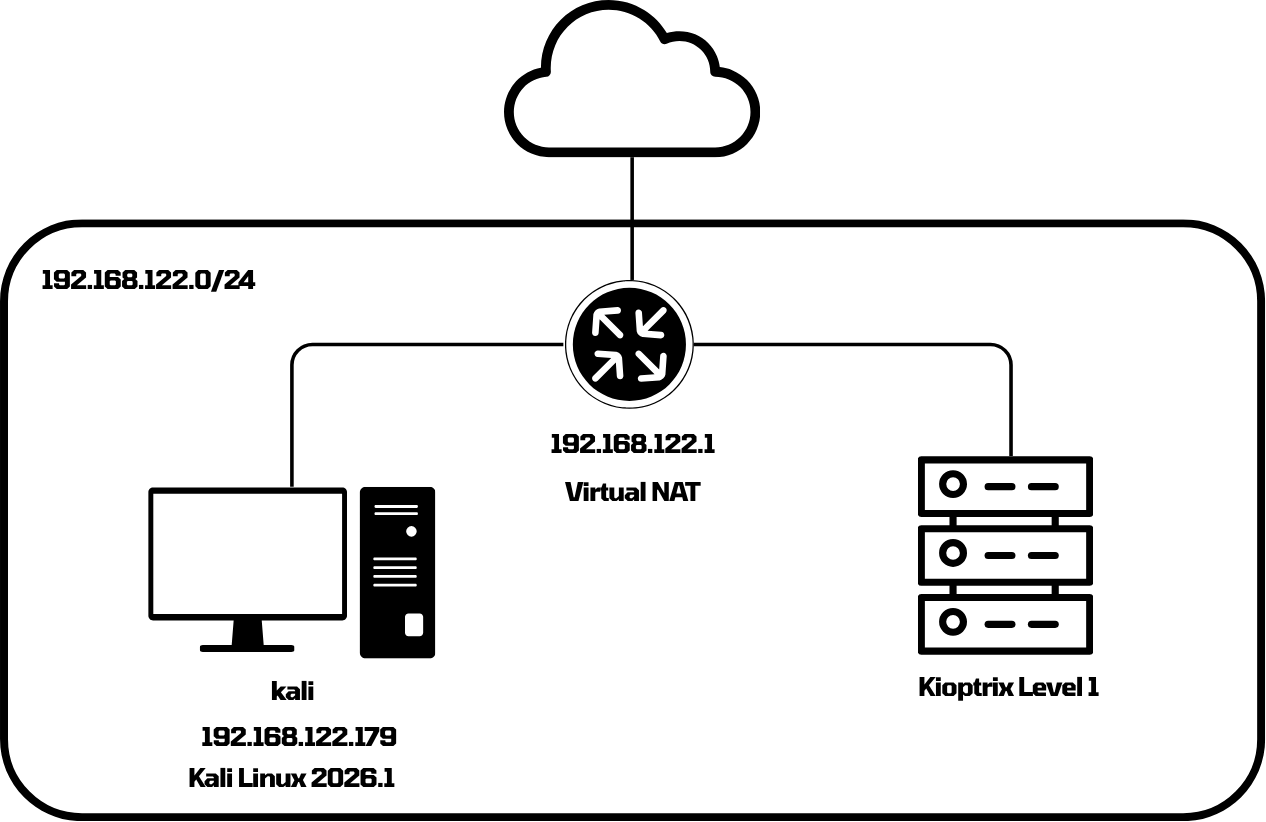
\includegraphics[width=0.9\textwidth]{assets/diagrammaRete.png}{Diagramma dell'architettura della rete virtuale.}
	
	Si è installata, in questa rete, una macchina virtuale Kali Linux 2026.1 tramite l'immagine di installazione ufficiale. La configurazione per la macchina Kali non ha richiesto passi particolari, trattandosi della configurazione di default consigliata da QEMU. In modo simile, è stata installata la macchina vulnerabile Kioptrix Level 1 tramite l'immagine pubblicata sul sito VulnHub\cite{vulnhub}. Si fa nota che la macchina Kioptrix, a causa delle datate richieste hardware, è stata configurata con:
	\begin{itemize}
		\item chipset della scheda madre di modello i440FX;
		\item bootloader di categoria BIOS;
		\item un disco virtuale simulato come tecnologia IDE;
		\item una scheda di rete del modello \emph{rtl8139}.
	\end{itemize}
	
	La macchina target Kioptrix Level 1 è stata configurata dopo l'installazione, per permettere al sistema operativo di configurare l'hardware emulato. Questo step è stato l'unico caso di accesso diretto alla macchina vulnerabile, mentre il resto dell'attività di attacco è stato svolto con metodologia \emph{black box}, senza conoscere alcun dettaglio particolare riguardo all'obiettivo, incluso l'indirizzo IP (fornito dal server DHCP simulato posto all'indirizzo 192.168.122.1) e l'indirizzo MAC della scheda di rete.
	
	\subsection{Strumenti utilizzati}
	Al fine dello svolgimento dell'attività di Penetration Testing, durante tutte le fasi sono stati utilizzati:
	\begin{itemize}
		\item il sistema di virtualizzazione QEMU basato su tecnologia KVM, configurato graficamente con VirtManager sull'host dell'ambiente di laboratorio (Pop\_OS! 24.04 LTS);
		\item gli strumenti forniti di default sulla macchina Kali Linux 2026.1, come \emph{nmap}\cite{nmap} e \emph{gobuster}\cite{gobuster};
		\item OpenVAS by Greenbone\cite{openvas} e Tenable Nessus Scanner\cite{nessus} (con licenza gratuita) installati sulla macchina Kali Linux al fine di effettuare una scansione remota approfondita della macchina target;
		\item browser web Firefox per la navigazione online e verso la VM;
		\item strumenti di ricerca online per l'information gathering, quali motore di ricerca DuckDuckGo, Google e il database di archiviazione di pagine "Web Archive: Wayback Machine"\cite{waybackmachine};
		\item risorsa online per l'ottenimento degli script di exploit per le diverse vulnerabilità individuate, ExploitDB\cite{exploitdb}.
	\end{itemize}
	
	\newpage
	\section{Target Scoping}
	Nel contratto di commissione del progetto, è stato fornito al team di Penetration Testing un link web alla pagina della macchina vulnerabile "Kioptrix: Level 1", contenente sia il link per l'installazione della VM, sia delle informazioni generali sull'autore della VM e un link ad una pagina blog riguardante la macchina vulnerabile.
	
	La fase di Target Scoping è stata segnata dallo studio delle regole di engagement, trattate nel report di attività di Penetration Testing, configurazione del laboratorio di test e progettazione dei passi da compiere con annessa installazione degli strumenti necessari.
	
	\subsection{Perimetro di lavoro}
	Dopo aver configurato la rete virtuale e la macchina Kali Linux, testiamo il corretto funzionamento dell'ambiente di laboratorio, controllando le informazioni di rete della macchina di penetration testing.
	
	\insertsvg[width=1.0\textwidth]{assets/ip_-c=never_address_1.svg}{Comando ip per ottenere le informazioni di rete.}
	
	Otteniamo l'indirizzo IP assegnato alla macchina Kali, 192.168.122.179, e possiamo confermare che essa è posizionata nella sottorete 192.168.122.0/24 come configurato. Nonostante non sia ancora noto l'indirizzo IP della macchina target, anch'essa ci si aspetta essere presente in questa rete.
	
	
	
	\newpage	
	\section{Information Gathering}
	\subsection{Passive gathering}
	Prima di provare ad ottenere informazioni in forma attiva interagendo via rete con la macchina target, si è deciso di sfruttare le informazioni pubblicamente disponibili riguardanti la VM per poter pianificare una strategia di attacco più mirata.
	
	La pagina web relativa alla macchina Kioptrix: Level 1 di VulnHub\cite{vulnhub} specifica il gruppo \emph{Kioptrix} come autore,
	e una pagina al sito \emph{kioptrix.com} come pagina di informazioni sulla macchina.
	
	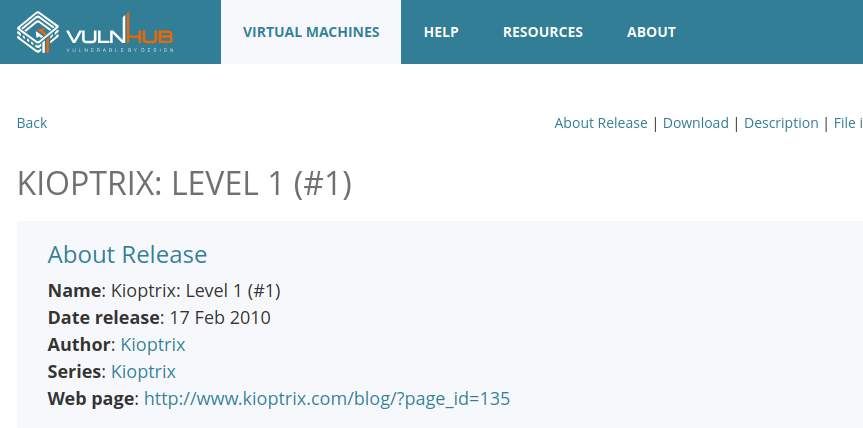
\includegraphics[width=0.9\textwidth]{assets/vulnhub.png}{Pagina relativa alla VM vulnerabile su vulnhub.com.}
	
	Provando ad accedere al link mostrato con Firefox, ci siamo accorti che il sito web kioptrix.com non è più raggiungibile in data odierna, motivo per cui iniziamo ad esplorare possibili archivi salvati sul WebArchive.
	
	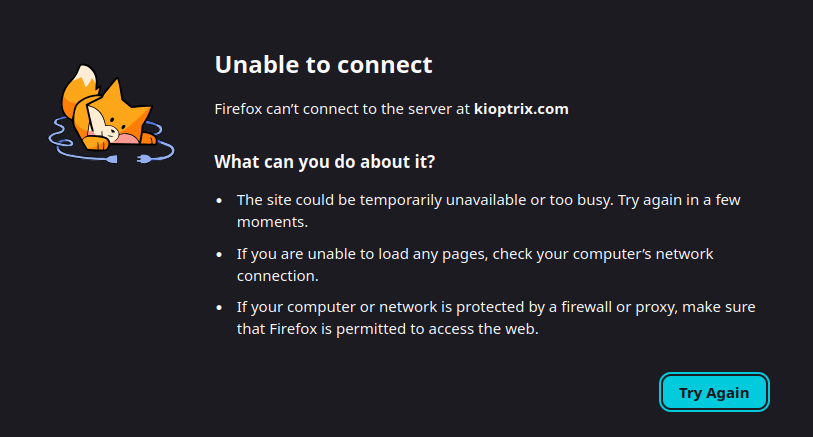
\includegraphics[width=0.8\textwidth]{assets/firefox-missing.png}{Errore di Firefox a causa della mancata connessione al sito kioptrix.com.}
	
	
\includegraphics[width=0.9\textwidth]{assets/wayback-machine-kioptrix.png}{Ricerca di archivi del sito di kioptrix.com su Wayback Machine.}
	
	\newpage
	L'ultimo archivio del blog kioptrix.com appartiene al 2017, e con esso riusciamo ad accedere alla pagina "About" che contiene i contatti dei membri del gruppo. Al contempo, però, scopriamo che la pagina relativa alla VM di interesse non è mai stata archiviata.
	
	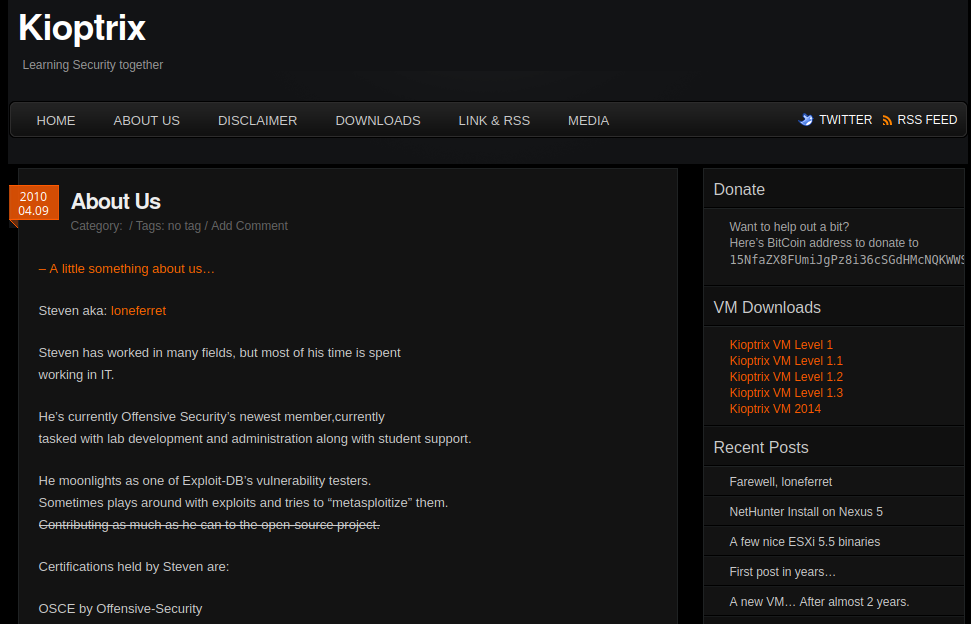
\includegraphics[width=0.9\textwidth]{assets/kioptrix-about.png}{Pagina "About" archiviata del blog kioptrix.com.}
	
	\subsection{Active gathering}
	Le tecniche di ricerca attiva delle informazioni sulla macchina sono state delegate alle fasi di Target Discovery e Service Mapping, a seconda delle necessità attuali e delle informazioni note in quel determinato momento.
	
	\newpage
	\section{Target Discovery}
	In questa fase del framework FGPT iniziamo a fare tentativi di rilevamento della macchina target, senza conoscerne le informazioni di rete. Poiché sappiamo avere la VM vulnerabile e la VM Kali nella medesima sottorete, possiamo pensare di ottenere le informazioni delle macchine collegate tramite una scansione ARP attiva.
	
	A questo fine, impieghiamo il comando \texttt{arp-scan}\cite{arpscan}.
	
	\insertsvg[width=1.0\textwidth]{assets/sudo_arp-scan_--localnet_1.svg}{Output del comando \texttt{arp-scan}.}
	
	Con l'opzione \texttt{---localnet} il comando \texttt{arp-scan} invia pacchetti in broadcast sulla sottorete locale e attende per le risposte con gli indirizzi IP assegnati. Nell'output del comando si possono vedere la macchina 192.168.122.1, cioè il router/NAT virtualizzato da QEMU per gestire la sottorete e un indirizzo IP sconosciuto, 192.168.122.85, che possiamo presupporre essere la macchina target.
	
	Per controllare il risultato di questa scansione, verifichiamo similmente con un altro strumento basato sul protocollo ARP chiamato \texttt{netdiscover}\cite{netdiscover}.
	
	\insertsvg[width=1.0\textwidth]{assets/sudo_netdiscover_-r_192.168.122.0_24_1.svg}{Output del comando \texttt{netdiscover}.}
	
	In questo caso, con precisione inferiore, lo strumento ha rilevato solo l'indirizzo IP della macchina vulnerabile, e non quello della macchina NAT.
	
	Come ultimo controllo, usiamo \texttt{nmap}\cite{nmap}, uno strumento capace di compiere scansioni ARP, IP e TCP/UDP, che sfrutteremo anche nelle fasi successive:
	
	\insertsvg[width=1.0\textwidth]{assets/nmap_-sn_192.168.122.0_24_1.svg}{Output del comando \texttt{nmap} con scansione ping locale.}
	
	\newpage
	In quest'ultimo caso, sfruttando l'opzione \texttt{--sn} che compie una scansione sulla sottorete specificata di sola discovery delle macchine, \texttt{nmap} ha rilevato sia la macchina vulnerabile, che il NAT (di cui ha anche correttamente menzionato il nome di dominio locale \texttt{pop-os.local}), che la macchina host \texttt{kali}, confermando definitivamente che questa è la configurazione completa della rete di laboratorio.
	
	Infine, per constatare con certezza che la macchina vulnerabile sia posta effettivamente nella medesima sottorete, sfruttiamo il comando \texttt{traceroute}\cite{traceroute} per poter calcolare il numero di hop (macchine/router attraversati) per raggiungere la macchina target.
	
	\insertsvg[width=1.0\textwidth]{assets/sudo_traceroute_192.168.122.85_1.svg}{Output del comando \texttt{traceroute} verso la macchina target.}
	
	L'output conferma un collegamento diretto, senza passare per il router della sottorete. Pertanto, la macchina target è effettivamente posta nella medesima sottorete.
	
	\newpage
	\section{Target Enumeration}
	La fase di Target Enumeration consiste nella scoperta dei servizi in esecuzione sulla macchina virtuale al fine di ottenere informazioni riguardo al suo utilizzo e poter mappare la superficie di attacco esposta.
	
	\subsection{Port Mapping}
	Al fine di scoprire quali porte di rete sono aperte (e quindi, si suppone, utilizzate) sfruttiamo diversi strumenti di scanning. Il funzionamento di questi strumenti, per le porte TCP, si basa sull'approccio SYN/ACK, per cui si spedisce un pacchetto TCP con una richiesta di connessione e si attende una risposta affermativa. Nonostante la connessione venga poi immediatamente troncata, la risposta del server implica che la porta a cui si è spedito il pacchetto sia effettivamente aperta.
	
	Tramite \texttt{masscan}\cite{masscan}, uno strumento pensato per poter scansionare migliaia di porte/host simultaneamente e in modo efficiente, otteniamo una prima lista delle porte aperte sulla macchina.
	
	\insertsvg[width=1.0\textwidth]{assets/sudo_masscan_192.168.122.85_-p0-65535_--rate_10000_1.svg}{Output del comando \texttt{masscan} verso la macchina target.}
	
	Nel range di tutte le 65535 porte possibili, sono state rilevate 6 porte aperte, di cui 5 \emph{IANA well-known} (nel range 0-1024) e una nel range di porte registrate.
	Controlliamo la scansione anche tramite l'uso del comando \texttt{nmap}.
	
	\insertsvg[width=0.9\textwidth]{assets/nmap_192.168.122.0_24_1.svg}{Output del comando \texttt{nmap} con scansione delle porte aperte.}
	
	L'esecuzione del comando \texttt{nmap} senza argomenti, che implica una scansione delle porte sulla sottorete, mostra le stesse 6 porte della VM target seguite dal relativo nome IANA. Possiamo quindi constatare con elevata sicurezza che le seguenti porte siano effettivamente aperte e che non ce ne siano altre aperte non rilevate.
	
	A questo punto è possibile stimare i servizi attivi nell'effettivo sul sistema (Web Server, SSH e Samba Network Share) grazie alle porte well-known, difficilmente utilizzate per altri scopi. Riguardo alla porta 32768, la cui funzione è registrata (ma non necessariamente deve trattarsi di quella specificata, diversamente dalle porte well known), si devono svolgere ulteriori scansioni per scoprirne l'uso.
	
	\subsection{Service Enumeration}
	Al fine di confermare le aspettative riguardo i servizi attivi sulla macchina vulnerabile e poter ottenere delle informazioni riguardanti i software che provvedono tali servizi (quali nome, versione etc.) eseguiamo una scansione approfondita di \texttt{nmap} sulle porte scoperte che effettua l'esecuzione di diversi script di riconoscimento dei servizi.
	
	\insertsvg[width=1.0\textwidth]{assets/nmap_-sV_-sS_-p22,80,111,139,443,32768_192.168.122.85_1.svg}{Output del comando \texttt{nmap} con riconoscimento dei servizi.}
	
	Oltre a specificare l'host target in particolare, e non più la sottorete, con le diverse porte rilevate (con opzione \texttt{--p}), sono state usate le flag \texttt{--sS}, per indicare la scansione di sole porte TCP, e \texttt{--sV}, per ottenere la versione dei servizi effettivamente utilizzati.
	
	La scansione conferma l'effettiva presenza dei diversi servizi nelle porte well-known, quali OpenSSH, Apache HTTPd e Samba\cite{samba}, il quale offre servizi nelle diverse porte fino alla 32768, come porta di status (\texttt{statmon2}).
	
	\subsection{Operating System Fingerprinting}
	Al fine di poter concludere l'analisi della macchina e poter passare alla ricerca effettiva delle vulnerabilità, è necessario individuare quale versione di sistema operativo è in esecuzione sulla macchina target.
	
	Questa ricerca è stata suddivisa in due fasi: fingerprinting passivo del sistema operativo, sfruttando tecniche e strumenti di riconoscimento del sistema remoto senza interazioni particolari col sistema, analizzando le risposte naturalmente offerte alle richieste dei servizi; fingerprinting attivo, stimolando volutamente il sistema (in modo più forzato e rilevabile) al fine di restringere il campo di possibili versioni dell'OS.
	
	\subsubsection{Fingerprinting Passivo}
	Per compiere una identificazione passiva del sistema operativo, sfruttiamo i diversi comportamenti del protocollo TCP della macchina target durante una semplice connessione HTTP. Quindi, in due sessioni parallele della shell di sistema, eseguiamo il comando \texttt{p0f}\cite{p0f}, che compie la scansione dei pacchetti in ingresso e uscita, ed eseguiamo \texttt{curl}\cite{curl}, un comando per compiere richieste HTTP a pagine web remote.
	
	\insertsvg[width=1.0\textwidth]{assets/curl_-G_192.168.122.85_1.svg}{Output del comando \texttt{curl} per la richiesta GET della pagina web.}
	
	Dopo aver aperto la sessione \texttt{p0f} eseguiamo \texttt{curl} con l'opzione \texttt{--G} per specificare di voler compiere una richiesta con metodo HTTP GET verso la VM target.
	In risposta, otteniamo una pagina \texttt{html} all'apparenza di "Test" per "Apache Web Server on Red Hat Linux".
	
	Se tali informazioni fossero attendibili, staremmo interagendo con una macchina Linux della distribuzione Red Hat. Inoltre, che la pagina appartenga al web server Apache conferma l'informazione ottenuta durante la scansione dei servizi.
	
	\newpage
	\insertsvg[width=1.0\textwidth]{assets/sudo_p0f_-i_eth0_1.svg}{Output del comando \texttt{p0f} con analisi dei pacchetti spediti.}
	
	Durante la richiesta HTTP, la sessione \texttt{p0f} ha scansionato i pacchetti in ingresso e in uscita sulla interfaccia di rete \texttt{eth0} (specificata con opzione \texttt{--i}). Visionando le scansioni per i pacchetti di apertura della connessione TCP, constatiamo che il kernel rilevato è di versione Linux 2.4.x, mentre la versione del server web dovrebbe trattarsi di Apache 1.3.20 con OpenSSL 0.9.6b, esattamente come rilevato durante la scansione dei servizi.
	
	\subsubsection{Fingerprinting Attivo}
	Cerchiamo di restringere il campo sfruttando script di riconoscimento del sistema operativo più precisi ma di tipologia attiva, facendo richiesta di informazioni specifiche al fine di appurare la versione specifica dell'OS. Anche per quest'uso, lo strumento \texttt{nmap} possiede un opzione apposita, attivata con argomento \texttt{-O}.
	
	\insertsvg[width=0.9\textwidth]{assets/nmap_-sS_-O_192.168.122.85_1.svg}{Output del comando \texttt{nmap} con riconoscimento dell'OS.}
	
	Questa scansione ha riconfermato il risultato di \texttt{p0f}, per cui il kernel è di versione 2.4.x, restringendo ulteriormente il campo tra le versioni 2.4.9 e 2.4.18. Con questo intervallo di versioni kernel e cercando online sui kernel utilizzati da RedHat Linux, riusciamo ad identificare, con buona affidabilità, che la macchina con cui stiamo avendo a che fare sia una RedHat Linux 7.2.
	
	\subsection{Topologia Web}
	Nota la presenza di un web server, decidiamo di esplorare le diverse pagine web disponibili al fine di comprendere l'uso della macchina e cercare per informazioni aggiuntive che potrebbero rivelare vettori di attacco.
	
	Un semplice accesso con Firefox verso l'indirizzo IP della macchina attaccata rivela la pagina di test ottenuta testualmente in precedenza.
	
	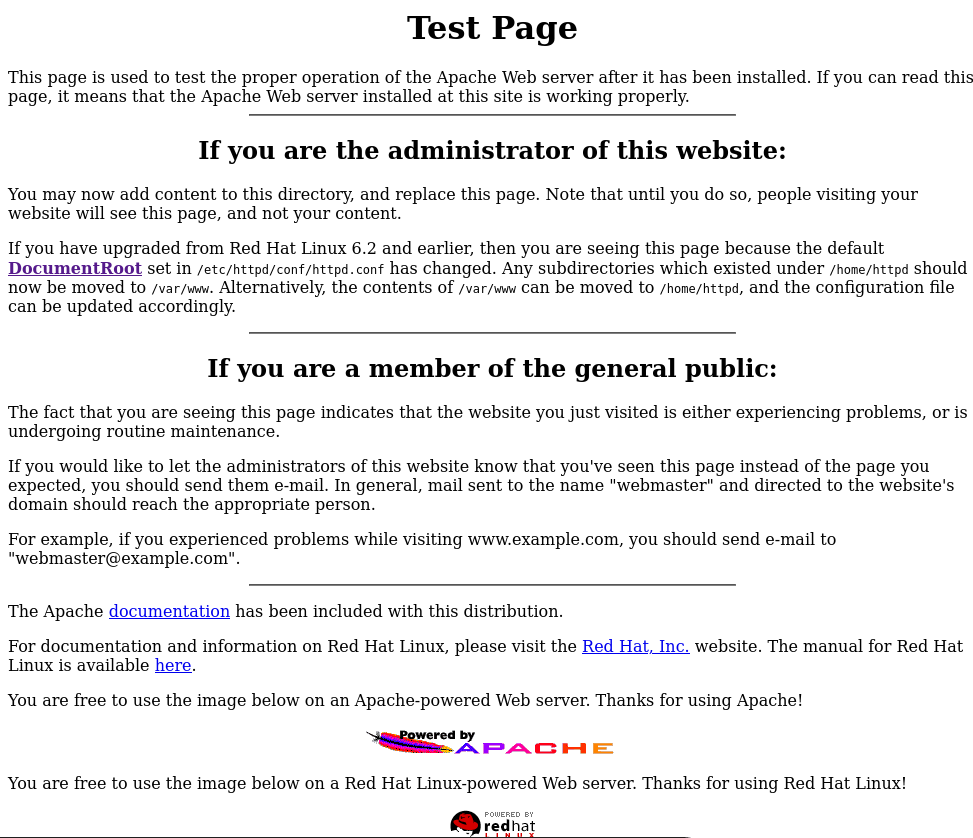
\includegraphics[width=1.0\textwidth]{assets/test-page.png}{Pagina di test ottenuta dalla richiesta HTTP verso la VM target.}
	
	Sfruttiamo il comando \texttt{gobuster}\cite{gobuster} per compiere un attacco a dizionario sul web server e cercare ogni pagina web liberamente accessibile.
	
	\insertsvg[width=1.0\textwidth]{assets/gobuster_dir_--url_192.168.122.85_--wordlist__usr_share_wordlists_dirb_big.txt_--delay_2ms_1.svg}{Output del comando \texttt{gobuster} che mostra i file presenti sul webserver attaccato.}
	
	\newpage
	Con l'opzione \texttt{---wordlist} è stata specificato un dizionario di file comunemente presenti in webserver tra cui cercare, in questo caso la wordlist \texttt{dirb/big.txt} presente di default su Kali Linux 2026.
	
	Possiamo vedere che esistono diversi file, nonostante siano tutti o inacessibili (errore 403) o ridirezionano alla rete di \emph{loopback} 127.0.0.1. Pertanto, anche tali file sono inacessibili dall'esterno, e in ogni caso si tratta di file di manuali o utilizzo del web server.
	
	È possibile accedere ai file con ridirezione ingannando il server web a credere che l'host richiedente sia 127.0.0.1, specificando l'header \texttt{Host: 127.0.0.1} durante la richiesta.			
	
	\insertsvg[width=1.0\textwidth]{assets/curl_-H_Host__127.0.0.1_http___192.168.122.85_usage_____usage.html_1.svg}{Output del comando \texttt{curl} per richiedere la pagina \texttt{usage} non normalmente accessibile.}
	
	Di seguito è visualizzata la pagina di Webalizer al percorso \texttt{/usage/} accessibile sfruttando questo metodo.
	
	\newpage
	
	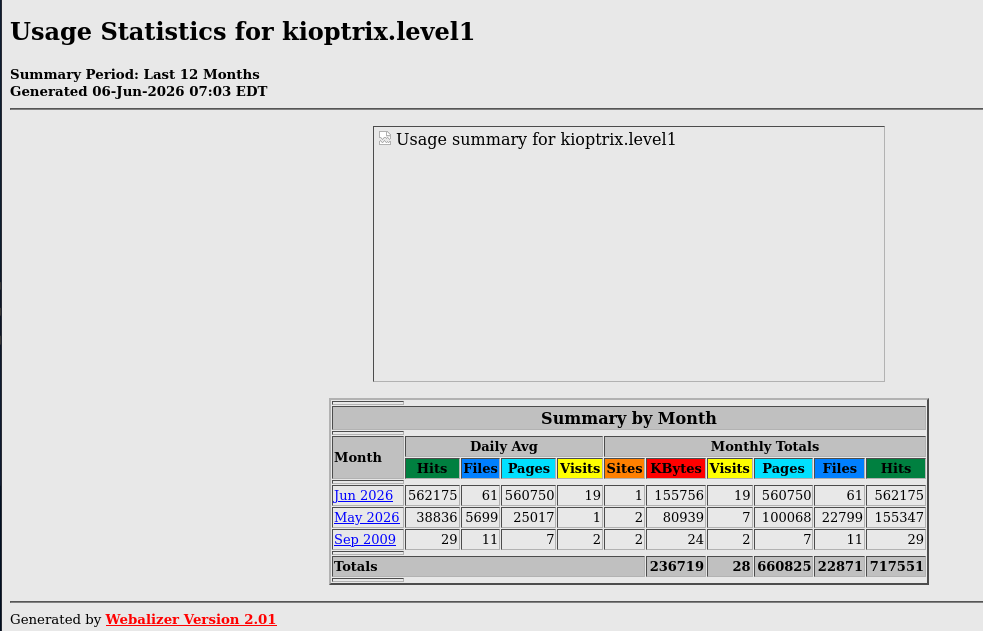
\includegraphics[width=0.9\textwidth]{assets/webalizer.png}{Pagina di Webalizer visualizzata al percorso \texttt{/usage/}.}
	
	Nonostante siano presenti delle pagine, si tratta di un webserver non configurato e senza pagine esposte dal creatore della VM. Le pagine di manuale dei moduli, Webalizer e di installazione di MRTG non contengono alcuna informazione o vulnerabilità sfruttabile.
	
	\subsection{Architettura di rete scansionata}
	Con le informazioni ottenute tramite le prime 4 fasi del framework FGPT, possiamo ora stilare un diagramma di rete completo con le informazioni sulla macchina attaccata e sui servizi che espone.
	
	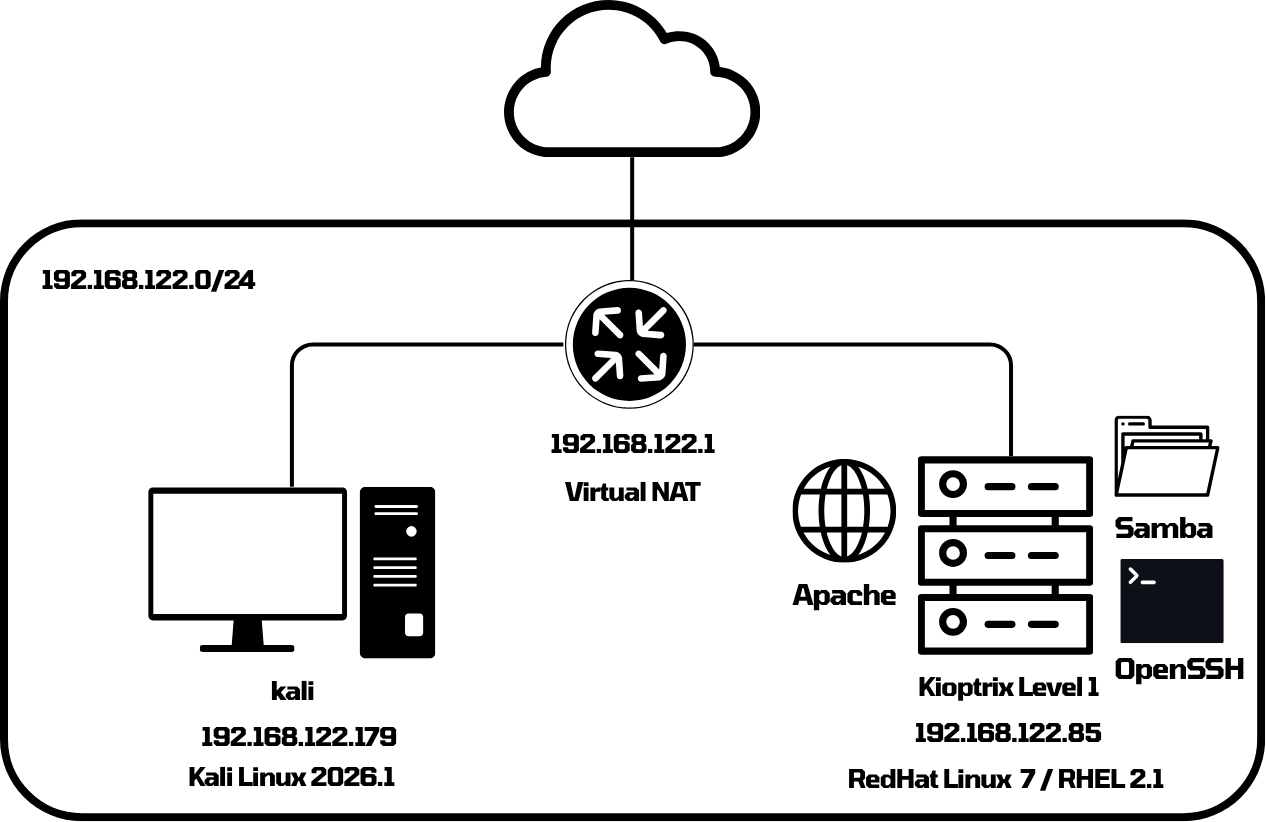
\includegraphics[width=0.75\textwidth]{assets/diagrammaReteFinale.png}{Architettura di rete nota al termine della scansione della macchina attaccata.}
	
	\newpage
	\section{Vulnerability Analysis}
	Una volta scoperte le informazioni identificative della macchina target e i servizi da essa esposti, si è fatto uso di tali informazioni per ricercare possibili vulnerabilità note da poter sfruttare nelle fasi successive del framework FGPT.
	
	\subsection{Scansioni Automatiche}
	Si è fatto uso degli strumenti di vulnerability scanning installati al fine di compiere analisi automatiche sulla macchina attaccata. Tutte le scansioni relative ai servizi attivi sono state compiute con copertura totale delle porte della macchina, seppur le analisi precedenti avessero già ristretto il campo di ricerca.
	
	Al termine delle eventuali scansioni sono stati recuperati i report dei risultati ottenuti come guida per la ricerca di vulnerabilità critiche e da cui difendersi.
	
	\subsubsection{OpenVAS}
	OpenVAS by Greenbone\cite{openvas} è stato configurato per compiere una scansione di rete profonda della macchina, su tutte le porte e per tutti i servizi disponibili.
	
	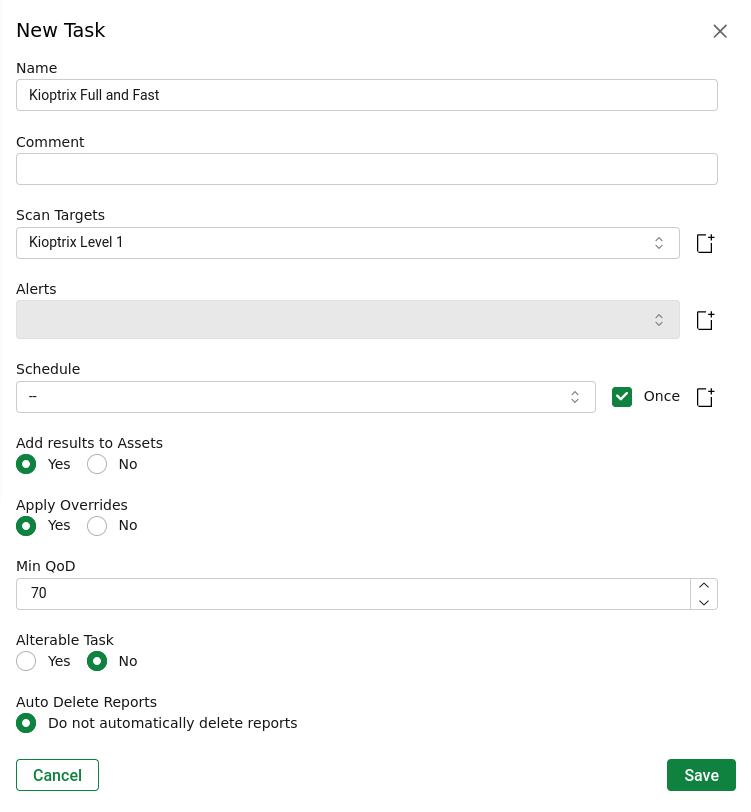
\includegraphics[width=0.70\textwidth]{assets/openvas-conf.png}{Wizard di configurazione di OpenVAS per la scansione completa.}
	
	La scansione ha avuto successo con oltre 29 vulnerabilità uniche rilevate. Le porte rilevate e i servizi associati erano i medesimi delle scansioni eseguite in precedenza. 
	
	\insertsvg[width=0.5\textwidth]{assets/openvas-chart.svg}{Diagramma a torta del numero di vulnerabilità rilevate da OpenVAS.}
	
	\begin{table}[htbp]
		\centering
		\small
		\begin{tabular}{|p{5.2cm}|c|c|p{1.8cm}|p{2.8cm}|}
			\hline
			\textbf{Vulnerabilità} & \textbf{Sev.} & \textbf{CVSS} &
			\textbf{Porta} & \textbf{CVE} \\
			\hline
			Deprecated SSH-1 Protocol Detection
			& High & 7.5 & 22/tcp & CVE-2001-0361\cite{cve-2001-0361} \\
			\hline
			Webalizer Cross-Site Scripting
			& High & 7.5 & 80, 443/tcp & CVE-2001-0835\cite{cve-2001-0835} \\
			\hline
			SSL/TLS Vulnerable Cipher Suites HTTPS (SWEET32)
			& High & 7.5 & 443/tcp & CVE-2016-2183\cite{cve-2016-2183} \\
			\hline
			SSL/TLS Weak Cipher Suites Supported
			& Medium & 5.9 & 443/tcp & CVE-2013-2566\cite{cve-2013-2566} \\
			\hline
			SSL/TLS Deprecated SSLv2 and SSLv3 Detection
			& Medium & 5.9 & 443/tcp & CVE-2016-0800\cite{cve-2016-0800} \\
			\hline
			HTTP TRACE/TRACK Debugging Methods Enabled
			& Medium & 5.8 & 80, 443/tcp & CVE-2003-1567\cite{cve-2003-1567} \\
			\hline
			Apache HTTP Server UserDir Information Disclosure
			& Medium & 5.0 & 80, 443/tcp & CVE-2001-1013\cite{cve-2001-1013} \\
			\hline
			SSL/TLS RSA\_EXPORT Downgrade (FREAK)
			& Medium & 4.3 & 443/tcp & CVE-2015-0204\cite{cve-2015-0204} \\
			\hline
		\end{tabular}
		\caption{Le 8 vulnerabilità di maggiore severità rilevate da OpenVAS.}
	\end{table}
	
	\subsubsection{Nessus Basic Scan}
	Tenable Nessus\cite{nessus} è stato utilizzato per due scansioni: una basic delle porte/servizi di rete sulla macchina; una incentrata sulle tecnologie web utilizzate, poiché nota la presenza di un server HTTP.
	
	La configurazione utilizzata ha avuto la seguente modalità:
	
	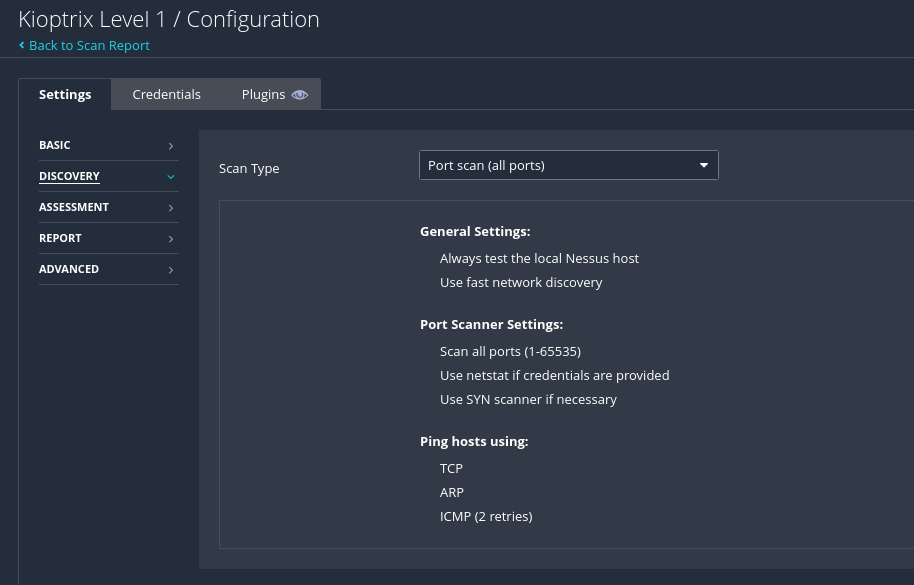
\includegraphics[width=0.62\textwidth]{assets/nessus-conf.png}{Configurazione di Nessus per la scansione basic.}
	
	Il risultato della scansione ha confermato 42 vulnerabilità uniche.
	
	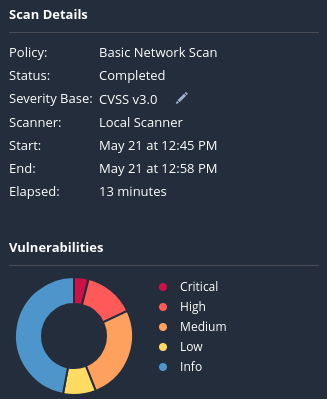
\includegraphics[width=0.25\textwidth]{assets/nessus-scan.png}{Diagramma a torta del numero di vulnerabilità rilevate da Nessus Basic Scan.}
	
	\begin{table}[htbp]
		\centering
		\small
		\begin{tabular}{|p{6cm}|c|c|p{1.8cm}|}
			\hline
			\textbf{Vulnerabilità} & \textbf{Sev.} & \textbf{CVSS} &
			\textbf{Porta} \\
			\hline
			OpenSSH $<$ 3.1 Channel Code Off-by-One Privilege Escalation
			& Critical & 10.0\textsuperscript{*} & 22/tcp \\
			\hline
			OpenSSH $<$ 3.4 Multiple Remote Overflows
			& Critical & 10.0\textsuperscript{*} & 22/tcp \\
			\hline
			OpenSSH $<$ 3.7.1 Multiple Vulnerabilities
			& Critical & 10.0\textsuperscript{*} & 22/tcp \\
			\hline
			OpenSSH $<$ 7.2 Untrusted X11 Forwarding Fallback
			& Critical & 9.8 & 22/tcp \\
			\hline
			SSL Version 2 and 3 Protocol Detection
			& Critical & 9.8 & 443/tcp \\
			\hline
			OpenSSH $<$ 10.3 Multiple Vulnerabilities
			& High & 8.1 & 22/tcp \\
			\hline
			OpenSSH $<$ 7.3 Multiple Vulnerabilities
			& High & 7.8 & 22/tcp \\
			\hline
			SSL Medium Strength Cipher Suites (SWEET32)
			& High & 7.5 & 443/tcp \\
			\hline
		\end{tabular}
		\caption{Le 8 vulnerabilità di maggiore severità rilevate da Nessus Basic
			Scan. \textsuperscript{*}~Punteggio CVSSv2 (CVSSv3 non disponibile).}
	\end{table}
	
	\newpage
	\subsubsection{Nessus Web Scan}
	La configurazione utilizzata ha avuto la seguente modalità:
	
	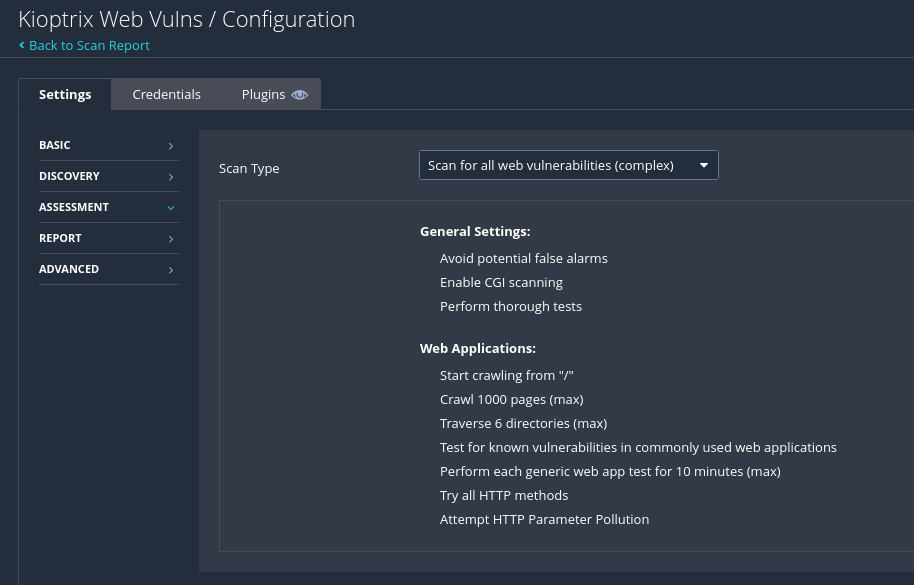
\includegraphics[width=0.62\textwidth]{assets/nessus-web-conf.png}{Configurazione di Nessus per la scansione web.}
	
	Il risultato della scansione ha confermato 14 vulnerabilità uniche.
	
	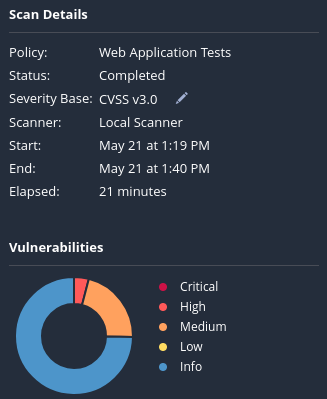
\includegraphics[width=0.25\textwidth]{assets/nessus-web.png}{Diagramma a torta del numero di vulnerabilità rilevate da Nessus Basic Scan.}
	
	\begin{table}[htbp]
		\centering
		\small
		\begin{tabular}{|p{6.5cm}|c|c|p{1.8cm}|}
			\hline
			\textbf{Vulnerabilità} & \textbf{Sev.} & \textbf{CVSS} & \textbf{Porta} \\
			\hline
			Apache Chunked Encoding Remote Overflow
			& High & 7.3 & 80/tcp \\
			\hline
			Web Server Generic XSS & Medium & 6.1 & 80/tcp \\
			\hline
			Apache Server ETag Header Information Disclosure
			& Medium & 5.3 & 80/tcp \\
			\hline
			Browsable Web Directories & Medium & 5.3 & 80/tcp \\
			\hline
			HTTP TRACE/TRACK Methods Allowed
			& Medium & 5.3 & 80/tcp \\
			\hline
			Webalizer $<$ 2.01-09 Multiple XSS
			& Medium & 4.3\textsuperscript{*} & 80/tcp \\
			\hline
		\end{tabular}
		\caption{Vulnerabilità classificate rilevate da Nessus Web Scan.
			\textsuperscript{*}~Punteggio CVSSv2 (CVSSv3 non disponibile).}
	\end{table}
	
	\newpage
	\subsubsection{Nikto}
	Lo strumento Nikto\cite{nikto} ha permesso un ulteriore scansione delle vulnerabilità web, ottenendo risultati simili (e meno profondi) della scansione con Nessus Web Scan.
	
	\insertsvg[width=1.0\textwidth]{assets/nikto_-host_192.168.122.85_1.svg}{Output del comando \texttt{nikto} con analisi del webserver attaccato.}
	
	Anche questo strumento ha rilevato la presenza di Webalizer, noto per essere debole ad attacchi di carattere XSS. Tuttavia, essendo le pagine di Webalizer schermate dalla connessione esterna diretta, è impossibile sfruttare tali vulnerabilità.
	
	\subsection{Ricerca Manuale}
	Oltre alle vulnerabilità rilevate tramite scansione automatica, è stata effettuata anche una ricerca manuale basandosi sulle versioni dei servizi e del sistema operativo rilevato.
	
	\subsubsection{Assessment Samba}
	Mancando delle credenziali di accesso al servizio Samba, lo strumento OpenVAS ha evitato ogni scansione del network share SMB, per cui le informazioni a riguardo sono state considerate scarseggianti. Nonostante anche Nessus non avesse rilevato la versione del server remoto SMB e possibili vulnerabilità, ha rilevato come non fosse necessario procedere con l'autenticazione al fine di collegarsi al server remoto.
	
	Con questa informazione, è stato tentato un approccio diretto da parte del team di Penetration Testing per verificare se fossero presenti vulnerabilità al server Samba non rilevate dagli strumenti automatici.
	
	Il primo passo è stato il tentato collegamento al server tramite lo strumento \texttt{rpcclient}\cite{samba}.
	
	\insertsvg[width=0.8\textwidth]{assets/rpcclient_-U____192.168.122.85_1.svg}{Output del comando \texttt{rpcclient} con analisi del Samba server attaccato.}
	
	\newpage
	Con l'opzione \texttt{--U ""} si indica la mancanza di un nome utente per l'autenticazione, e anche la password è stata lasciata vuota al prompt. Come si vede dall'output del comando, le specifiche di sicurezza per la password sono nulle e il server non mostra esplicitamente la versione su cui è eseguito alla richiesta di informazioni.
	
	Per proseguire con l'assessment della versione del Samba server, si è fatto uso di uno script di analisi compreso in \texttt{msfconsole}\cite{metasploit} atto a questo fine:
	
	\insertsvg[width=1.0\textwidth]{assets/cat_smb_version.txt_1.svg}{Output del comando \texttt{msfconsole} con analisi della versione del Samba server attaccato.}
	
	Ricercando la versione di Samba 2.2.1a su ExploitDB\cite{exploitdb}, veniamo a conoscenza di una vulnerabilità nota come \texttt{trans2open}, di CVSSv3 10.0, che aggiungiamo alla lista di vulnerabilità da dover controllare.
	
	\subsubsection{Assessment OS}
	Oltre ad un generico avviso di obsolescenza, notiamo una mancanza di scansioni di vulnerabilità relative al sistema operativo (ormai datato) sugli strumenti di scansione automatici, che ci porta a compiere ricerche basate sulla versione del kernel 2.4.x e della distribuzione RedHat Linux 7.2.
	
	Tramite una ricerca su ExploitDB, veniamo a conoscenza della vulnerabilità \texttt{ptrace-kmod}, una vulnerabilità di privilege escalation locale dovuta alla versione del kernel.
	
	\subsection{Risultati dell'assessment}
	In totale, sono state rilevate 76 vulnerabilità uniche raggruppando i risultati dei diversi strumenti.
	
	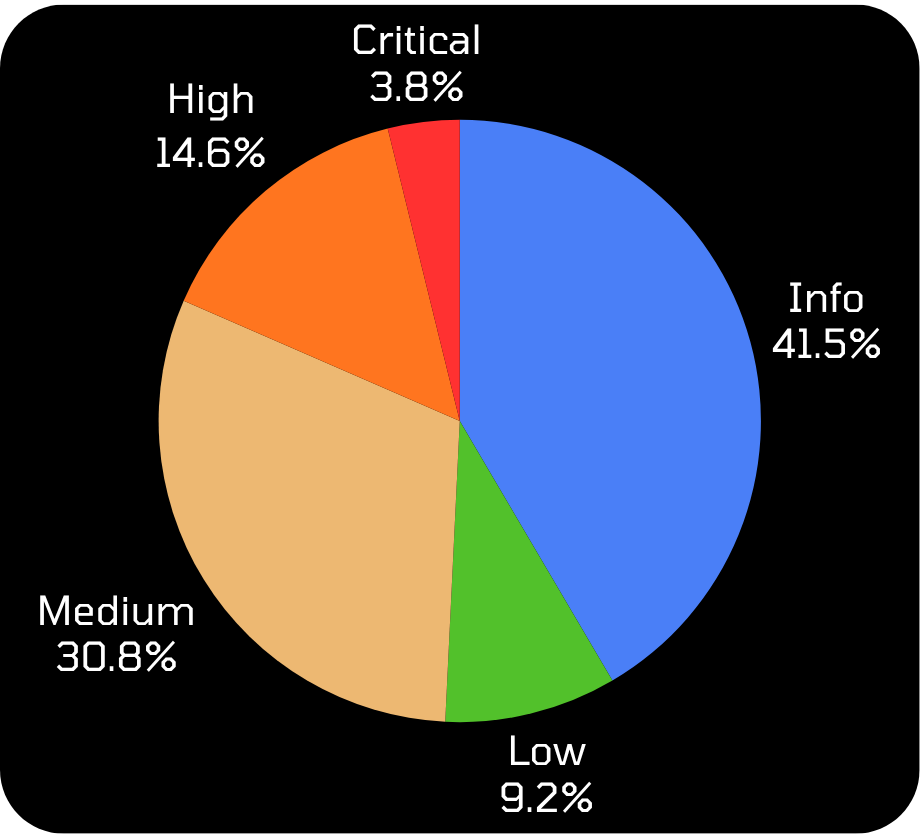
\includegraphics[width=0.5\textwidth]{assets/total-vulns.png}{Diagramma a torta del numero di vulnerabilità totali raggruppando le diverse fonti.}
	
	\newpage
	\section{Target Exploitation}
	\subsection{Vulnerabilità critiche di interesse}
	Ai fini dell'attività di exploitation, le vulnerabilità sfruttate sono state:
	\begin{itemize}
		\item \textbf{CVE-2002-0082}\cite{cve-2002-0082}, \texttt{open-ssl-too-open}
		\item \textbf{CVE-2003-0201}\cite{cve-2003-0201}, \texttt{trans2open}
		\item \textbf{CVE-2003-0127}\cite{cve-2003-0127}, \texttt{ptrace-kmod}
	\end{itemize}
	
	\subsection{Exploit trans2open}
	Per sfruttare la vulnerabilità \texttt{trans2open}, si è fatto uso degli script compresi in \texttt{msfconsole}\cite{exploit-trans2open}.
	
	\insertsvg[width=0.80\textwidth]{assets/cat_trans2open_search.txt_1.svg}{Ricerca dell'exploit per \texttt{trans2open} nel prompt di \texttt{msfconsole}.}
	
	Usiamo l'exploit di indice 2 (per Linux) verso l'IP della VM attaccata e impostiamo un payload con \texttt{reverse\_shell} per poter immettere comandi remoti.
	
	\insertsvg[width=0.9\textwidth]{assets/cat_exploit_trans2open.txt_1.svg}{Uso dell'exploit per \texttt{trans2open} nel prompt di \texttt{msfconsole}.}
	
	Possiamo verificare di aver ottenuto una shell remota con permessi \texttt{root}, così completando uno dei possibili percorsi di attacco per la macchina.
	
	\subsection{Exploit openssl-too-open}
	Per sfruttare la vulnerabilità \texttt{openssl-too-open} si è fatto uso dello script di exploit OpenFuckV3\cite{exploit-openfuck} presente su ExploitDB.
	
	Utilizzando \texttt{searchsploit}, un comando per navigare negli script di ExploitDB, con l'opzione \texttt{-m} si è scaricata in locale una copia dello script di exploit.
	
	\insertsvg[width=0.8\textwidth]{assets/searchsploit_-m_47080_1.svg}{Output del comando \texttt{searchsploit} per ottenere lo script \texttt{OpenFuckV3}.}
	
	Dopo aver scaricato il file, è necessario solo compilarlo con \texttt{gcc 47080.c -o openfuck -lcrypto} e eseguirlo con il codice \texttt{0x6b}, che indica la versione della macchina target (RedHat Linux 7.2 con Apache 1.3.20) e l'IP della macchina attaccata per permettere l'esecuzione dell'exploit.
	
	\insertsvg[width=0.8\textwidth]{assets/cat_openfuck_open.txt_1.svg}{Output dell'exploit script \texttt{OpenFuckV3} per ottenere accesso remoto alla macchina attaccata.}
	
	L'exploit ha successo e permette l'accesso ad una shell remota con permessi del server Apache (non amministratore). Per la cattura della flag è necessaria una strategia di privilege escalation locale.
	
	\section{Privilege Escalation}
	Poiché l'exploit sfruttando \texttt{trans2open} non richiede privilege escalation, accedendo alla macchina remota già come \texttt{root}, questa sezione continua dal lavoro svolto per l'exploit \texttt{open-ssl-too-open}, facendo uso della vulnerabilità critica \texttt{ptrace-kmod}. Anche in questo caso, prima di ogni altro passo, scarichiamo lo script di exploit\cite{exploit-ptrace} sulla macchina attaccante.
	
	\insertsvg[width=1.0\textwidth]{assets/searchsploit_-m_3_1.svg}{Output del comando \texttt{searchsploit} per ottenere lo script di exploit \texttt{ptrace-kmod}.}
	
	Questo script, scritto in linguaggio C, deve essere eseguito localmente alla macchina vulnerabile, e non da remoto. Pertanto, è necessario un mezzo di comunicazione del file tra macchina attaccante e macchina attaccata per permettere il trasferimento. Si fa uso di un semplice HTTP server temporaneo sulla macchina attaccante per condividere pubblicamente il file \texttt{3.c}.
	
	\insertsvg[width=1.0\textwidth]{assets/python_-m_http.server_8080_1.svg}{Apertura di un semplice server HTTP per la condivisione dello script di exploit \texttt{ptrace-kmod}.}
	
	Il comando visto sopra permette una condivisione alla porta 8080 dell'host Kali, che deve quindi ricevere una richiesta GET dalla macchina attaccata per permettere la condivisione.
	Quindi, una volta ottenuto l'accesso come utente \texttt{apache} tramite l'exploit remoto, usiamo il comando \texttt{wget} per scaricare il file dall'indirizzo IP della macchina Kali e lo compiliamo con il compilatore \texttt{gcc} presente sulla macchina.
	
	\insertsvg[width=0.95\textwidth]{assets/cat_openfuck_privesc.txt_1.svg}{Tecnica di privilege escalation sfruttando l'exploit \texttt{ptrace-kmod}.}
	
	Come si vede dall'output riportato sopra, l'exploit ha successo e otteniamo accesso come utente \texttt{root} sulla macchina remota.
	
	\newpage
	\section{Maintaining Access}
	\subsection{Backdoor setup}
	L'ultimo passo è quello di permettere un accesso persistente alla macchina da remoto anche dopo aver rimediato alle vulnerabilità scansionate e utilizzate.
	
	Indipendentemente dall'exploit utilizzato per ottenere accesso amministrativo da remoto sulla macchina, è possibile installare una semplice backdoor automatica e persistente sfruttando la configurazione di \texttt{cron}.
	
	\insertsvg[width=1.0\textwidth]{assets/cat_backdoor.txt_1.svg}{Configurazione della backdoor sfruttando una reverse shell avviata da \texttt{cron}.}
	
	Nella schermata riportata sopra si può vedere la configurazione di una reverse shell verso la macchina attaccante sulla porta 4444, eseguita ad intervalli di un minuto (configurazione temporale "* * * * *") come utente \texttt{root}.
	
	Ascoltando sulla porta 4444 dalla macchina Kali Linux con \texttt{netcat}, basta aspettare il cambio del minuto attuale per ricevere una richiesta di connessione con una shell remota pronta all'uso.
	
	\insertsvg[width=1.0\textwidth]{assets/nc_-lvnp_4444_1.svg}{Output di \texttt{netcat} alla shell di backdoor con accesso \texttt{root}.}
	
	\subsection{Detection artifacts}
	Con la fase di configurazione della backdoor, sul sistema attaccato è stato lasciato un file di configurazione \texttt{cron} alla posizione \texttt{/etc/cron.d/root}. Nel file in questione è quindi specificato l'indirizzo IP della macchina attaccante, permettendo comunque un grado di rintracciabilità elevato rispetto a backdoor realmente utilizzabili.
	
	\section{Considerazioni Finali}
	Il team ha configurato l'ambiente di laboratorio per testare la macchina virtuale Kioptrix: Level 1 come da commissione, permettendo una connessione simulata di una rete LAN.
	
	Tramite l'uso di tecnologie avanzate di Penetration Testing, il team è riuscito a recuperare informazioni online archiviate sulla macchina e sui suoi produttori, è riuscito a rilevare la VM sulla rete e ha iniziato una scansione delle porte di rete aperte e dei servizi disponibili.
	Procedendo sulla base delle informazioni raccolte, sono state effettuate scansioni mirate sulla macchina per possibili vulnerabilità sia con strumenti automatici che tramite ricerca manuale, a livello di rete o di operatività web.
	Analizzando attentamente i risultati del vulnerability assessment, sono state individuate le vulnerabilità più critiche e efficacemente utilizzabili nella fase di exploitation.
	Sono stati eseguiti exploit distinti e paralleli di diverse tecnologie, seguite da un eventuale fase di privilege escalation, così ottenendo l'obiettivo di controllo remoto sulla macchina come utente \texttt{root}.
	Infine, come aggiunta operativa, è stata posizionata una semplice backdoor persistente per poter accedere rapidamente alla macchina remota come amministratore.
	
	Il lavoro ha dimostrato essere molto efficaci gli exploit riguardanti buffer overflow presenti in librerie e servizi oramai obsoleti al tempo in cui tali vulnerabilità non erano comunemente controllate. Il sistema si è dimostrato estremamente indifeso per gli standard moderni, presentando decine di vulnerabilità di criticità variegata seppur facilmente utilizzabili poiché profondamente documentate e note in data odierna.
	
	\newpage
	\section{Bibliografia}
	
	\begin{thebibliography}{99}
		
		% ----- Macchina target e fonti di ricerca -----
		\bibitem{vulnhub}
		VulnHub, \emph{Kioptrix: Level 1 (\#1)},
		\url{https://www.vulnhub.com/entry/kioptrix-level-1-1,22/}
		
		\bibitem{waybackmachine}
		Internet Archive, \emph{Wayback Machine},
		\url{https://web.archive.org/}
		
		\bibitem{exploitdb}
		Offensive Security, \emph{Exploit Database (ExploitDB)},
		\url{https://www.exploit-db.com/}
		
		% ----- Strumenti Kali -----
		\bibitem{nmap}
		Kali Linux Tools, \emph{nmap},
		\url{https://www.kali.org/tools/nmap/}
		
		\bibitem{gobuster}
		Kali Linux Tools, \emph{gobuster},
		\url{https://www.kali.org/tools/gobuster/}
		
		\bibitem{masscan}
		Kali Linux Tools, \emph{masscan},
		\url{https://www.kali.org/tools/masscan/}
		
		\bibitem{arpscan}
		Kali Linux Tools, \emph{arp-scan},
		\url{https://www.kali.org/tools/arp-scan/}
		
		\bibitem{netdiscover}
		Kali Linux Tools, \emph{netdiscover},
		\url{https://www.kali.org/tools/netdiscover/}
		
		\bibitem{traceroute}
		Kali Linux Tools, \emph{traceroute},
		\url{https://www.kali.org/tools/traceroute/}
		
		\bibitem{p0f}
		Kali Linux Tools, \emph{p0f},
		\url{https://www.kali.org/tools/p0f/}
		
		\bibitem{curl}
		Kali Linux Tools, \emph{curl},
		\url{https://www.kali.org/tools/curl/}
		
		\bibitem{samba}
		Kali Linux Tools, \emph{samba (smbclient / rpcclient)},
		\url{https://www.kali.org/tools/samba/}
		
		\bibitem{metasploit}
		Kali Linux Tools, \emph{Metasploit Framework},
		\url{https://www.kali.org/tools/metasploit-framework/}
		
		\bibitem{nikto}
		Kali Linux Tools, \emph{nikto},
		\url{https://www.kali.org/tools/nikto/}
		
		% ----- Scanner di vulnerabilità -----
		\bibitem{openvas}
		Greenbone Networks, \emph{OpenVAS / Greenbone Vulnerability Management},
		\url{https://www.greenbone.net/en/family-of-solutions/}
		
		\bibitem{nessus}
		Tenable, \emph{Nessus Vulnerability Scanner},
		\url{https://www.tenable.com/products/nessus}
		
		% ----- CVE (National Vulnerability Database) -----
		\bibitem{cve-2001-0361}
		NVD, \emph{CVE-2001-0361},
		\url{https://nvd.nist.gov/vuln/detail/CVE-2001-0361}
		
		\bibitem{cve-2001-0835}
		NVD, \emph{CVE-2001-0835},
		\url{https://nvd.nist.gov/vuln/detail/CVE-2001-0835}
		
		\bibitem{cve-2016-2183}
		NVD, \emph{CVE-2016-2183},
		\url{https://nvd.nist.gov/vuln/detail/CVE-2016-2183}
		
		\bibitem{cve-2013-2566}
		NVD, \emph{CVE-2013-2566},
		\url{https://nvd.nist.gov/vuln/detail/CVE-2013-2566}
		
		\bibitem{cve-2016-0800}
		NVD, \emph{CVE-2016-0800},
		\url{https://nvd.nist.gov/vuln/detail/CVE-2016-0800}
		
		\bibitem{cve-2003-1567}
		NVD, \emph{CVE-2003-1567},
		\url{https://nvd.nist.gov/vuln/detail/CVE-2003-1567}
		
		\bibitem{cve-2001-1013}
		NVD, \emph{CVE-2001-1013},
		\url{https://nvd.nist.gov/vuln/detail/CVE-2001-1013}
		
		\bibitem{cve-2015-0204}
		NVD, \emph{CVE-2015-0204},
		\url{https://nvd.nist.gov/vuln/detail/CVE-2015-0204}
		
		\bibitem{cve-2002-0082}
		NVD, \emph{CVE-2002-0082},
		\url{https://nvd.nist.gov/vuln/detail/CVE-2002-0082}
		
		\bibitem{cve-2003-0201}
		NVD, \emph{CVE-2003-0201},
		\url{https://nvd.nist.gov/vuln/detail/CVE-2003-0201}
		
		\bibitem{cve-2003-0127}
		NVD, \emph{CVE-2003-0127},
		\url{https://nvd.nist.gov/vuln/detail/CVE-2003-0127}
		
		
		% ----- Exploit specifici -----
		\bibitem{exploit-trans2open}
		Exploit-DB, \emph{Samba trans2open Overflow (Linux x86)}, ID 7,
		\url{https://www.exploit-db.com/exploits/7}
		
		\bibitem{exploit-openfuck}
		Exploit-DB, \emph{Apache mod\_ssl < 2.8.7 OpenSSL - 'OpenFuckV2.c' Remote Buffer Overflow}, ID 47080,
		\url{https://www.exploit-db.com/exploits/47080}
		
		\bibitem{exploit-ptrace}
		Exploit-DB, \emph{Linux Kernel 2.2.x/2.4.x (RedHat) - 'ptrace/kmod' Local Privilege Escalation}, ID 3,
		\url{https://www.exploit-db.com/exploits/3}
		
	\end{thebibliography}
	
\end{document}